\documentclass[11pt,reqno,oneside,a4paper]{article}

\usepackage{amsmath}
\usepackage{amssymb}
\usepackage{amsthm}
\usepackage{graphicx}

\newtheorem{theorem}{Theorem}
\newtheorem{corollary}{Corollary}[theorem]
\newtheorem{lemma}[theorem]{Lemma}

\title{Teorema de Pitágoras}
\author{Daniela}
\date{\today}  


\begin{document}
\maketitle

\begin{theorem} \label{thm:Pitágoras}(Pitágoras)
	Suponha que um triângulo reto tenha hipotenusa de comprimento $c$ e catetos de comprimento $a$ e $b$. Segue-se que $c^2 = a^2 + b^2$.
\end{theorem}

\begin{proof}

Nós podemos organizar 4 desses triângulos da seguinte forma. Note que são formados dois quadriláteros:

%inserir imagem
\begin{figure}[htb]
	\centering
	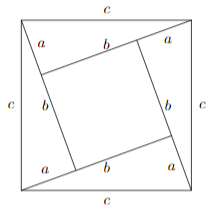
\includegraphics{pit.png}
	\label{fig: Pitágoras}
	\caption{Quatro cópias idênticas do triângulo organizadas de maneira que suas hipotenusas formem um quadrilátero que contém os quatro triângulos.}
\end{figure}

Os ângulos internos de um triângulo somam a $\pi$, mas o triângulo em questâo tem um ângulo reto, então os dois ângulos restantes somam a $\frac{\pi}{2}$. O quadrilátero externo é formado pela soma de um dos ângulos agudos de um triângulo e do outro ângulo agudo do outro triângulo. Portanto, esse quadrilátero externo é um retângulo. Além disso, como os triângulos são idênticos, todos têm a mesma hipotenusa, e os lados desse quadrilátero exterior são portanto todos iguais, fazendo desse quadrilátero um quadrado.
\\ \\
Como os triângulos são retos, o quadrilátero interno também tem ângulos retos. Além disso, cada lado do quadrilátero interno mede $(b-a)$, então o quadrilátero interno também é um quadrado.
\\ \\
O quadrado externo tem área $c^2$, o quadrado interno tem área $(b -a)^2$, e cada triângulo tem área $\frac{1}{2}ab$. Como o quadrado externo é formado pelo quadrado interno e mais quatro triângulos, temos:

$$c^2 = (b - a)^2 + 4 \times \frac{1}{2}(ab)$$
$$\Leftrightarrow c^2 = b^2 - 2ab + a^2 + \frac{4}{2}ab$$
$$\Leftrightarrow c^2 = a^2 +  b^2 - 2ab + 2ab$$
$$\Leftrightarrow c^2 = a^2 + b^2.$$

\end{proof}
\end{document} 
